\section{Appendix} \label{sec:appendix}

\subsection{\textit{UFRGS Entrance Exam and GPA} dataset}\label{sec:appendix1}

The following section contains the results considering the second dataset used for reproduction of the original experiments as described in section \ref{sec:datasets} and \ref{sec:experiments}. In this dataset sex is used as the fairness attribute, and race as the demographic attribute. 

The hyperparameters values used for these experiments are summarised in Table \ref{tab:brazil_hyperparams}.

\begin{table}[ht]
\centering
\footnotesize
    \begin{tabular}{l|c|c|c|c|c|c}
    Constraint & $\epsilon$ & train / test & Dc / Df & n-iters & $\delta$ & $\alpha$* \\\hline 
    DI & -0.8 & 0.4 & 0.4 &  2000 & 0.05 & 0.25\\
    DP & 0.1 & 0.4 & 0.4 & 2000 & 0.05 & 0.25 \\
    \end{tabular}
    \caption{Hyperparameter values for the experiments run with the \textit{UFRGS GPA} dataset specified for Disparate Impact (DI) or Demographic Parity (DP) for both a known and unknown demographic shift. $\alpha$ is only used in the case of an unknown shift.}
    \label{tab:brazil_hyperparams}
\end{table}

Shown in figure \ref{fig:brazil_k_shift} are the results under a known demographic shift with DP and DI as the fairness constraints. Results under unknown demographic shift considering DP and DI as the fairness constraints are shown in figure \ref{fig:brazil_unk_shift}.

\begin{figure}[ht]
    \begin{subfigure}{\linewidth}
      \centering
      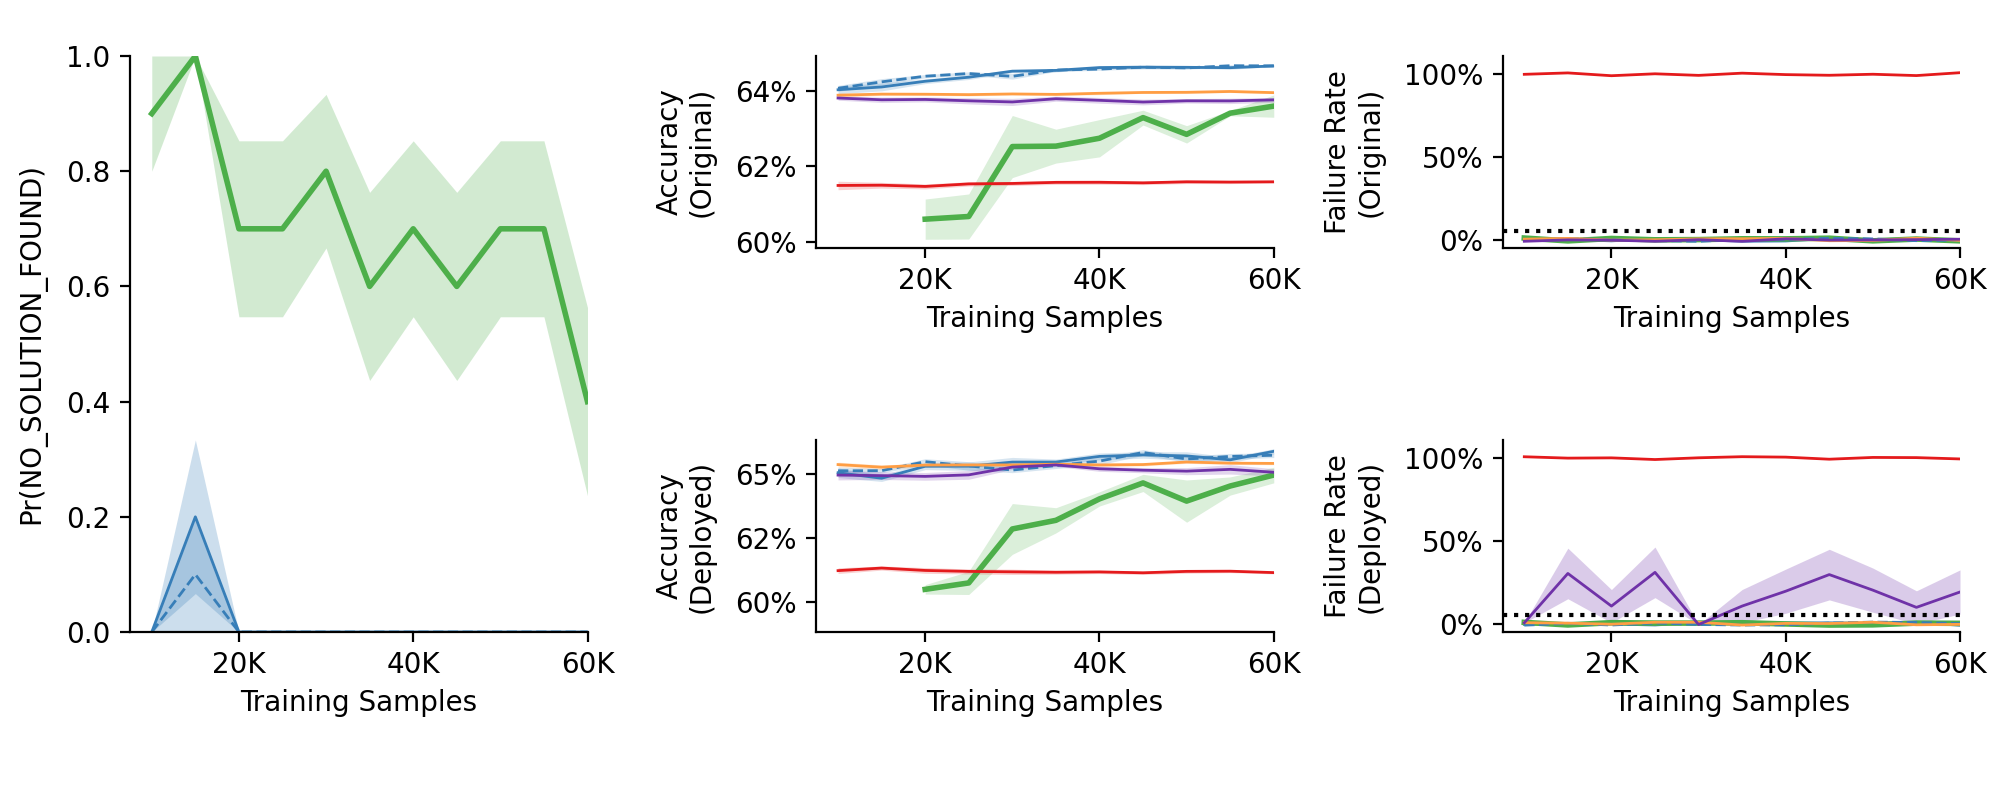
\includegraphics[scale=0.5]{figures/iclr_fixed_demographic_shift_brazil_rl/iclr_brazil_fixed_ds_rl_dp.png}
      \caption{Demographic Parity}
      \label{fig:brazil_k_dp}
    \end{subfigure}
    \begin{subfigure}{\linewidth}
      \centering
      \includegraphics[scale=0.5]{figures/iclr_fixed_demographic_shift_brazil_rl/iclr_brazil_fixed_ds_rl_di.png}
      \caption{Disparate Impact}
      \label{fig:brazil_k_di}
    \end{subfigure}
    \begin{subfigure}{\textwidth}
        \includegraphics[width=\linewidth]{figures/iclr_antag_demographic_shift_brazil_rl/iclr_legend.png}
    \end{subfigure}
    
    \caption{Results when enforcing fairness constraints under known demographic shift using the \textit{UFRGS GPA} dataset. For both fairness constraints DP and DI, the leftmost graph shows the probability of \texttt{NO\_SOLUTION\_FOUND}, the middle column shows the accuracies, and the rightmost column shows the failure rates.}
    \label{fig:brazil_k_shift}
\end{figure}



\begin{figure}[ht]
    \begin{subfigure}{\linewidth}
      \centering
      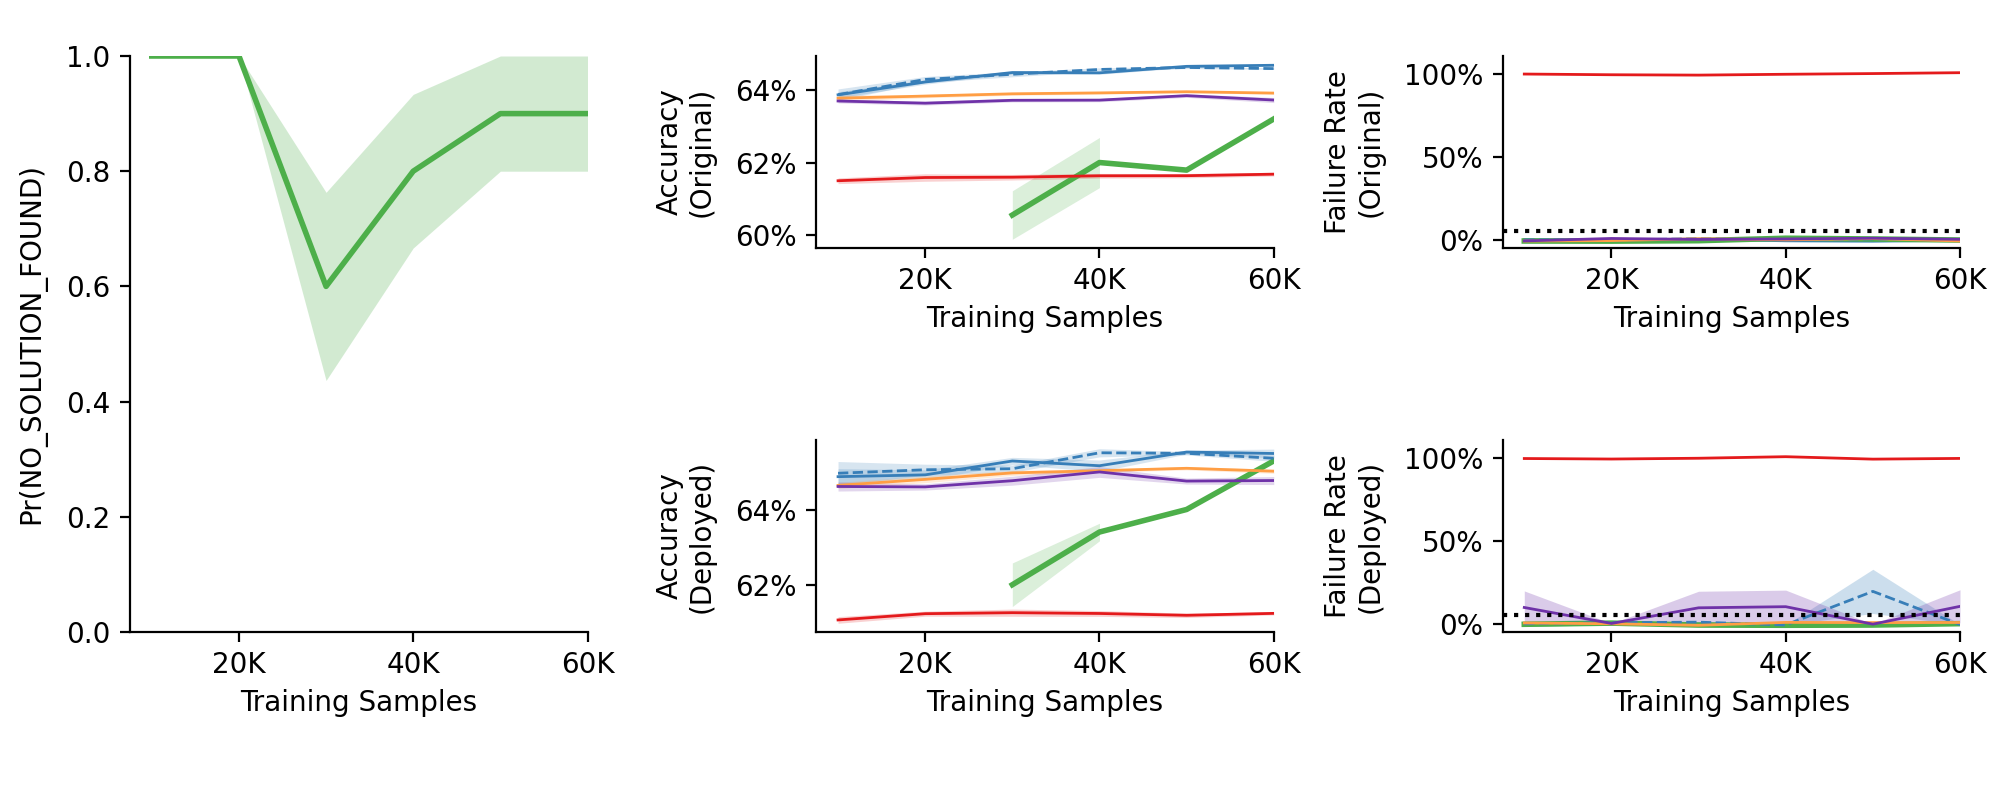
\includegraphics[scale=0.5]{figures/iclr_antag_demographic_shift_brazil_rl/iclr_brazil_antag_ds_rl_dp.png}
      \caption{Demographic Parity}
      \label{fig:brazil_unk_dp}
    \end{subfigure}
    \begin{subfigure}{\linewidth}
      \centering
      \includegraphics[scale=0.5]{figures/iclr_antag_demographic_shift_brazil_rl/iclr_brazil_antag_ds_rl_di.png}
      \caption{Disparate Impact}
      \label{fig:brazil_unk_di}
    \end{subfigure}
    \begin{subfigure}{\textwidth}
    \includegraphics[width=\linewidth]{figures/iclr_antag_demographic_shift_brazil_rl/iclr_legend.png}
    \end{subfigure}
    
    \caption{Results when enforcing fairness constraints under unknown demographic shift using the \textit{UFRGS GPA} dataset. For both fairness constraints DP and DI, the leftmost graph shows the probability of \texttt{NO\_SOLUTION\_FOUND}, the middle column shows the accuracies, and the rightmost column shows the failure rates.} 
    \label{fig:brazil_unk_shift}
\end{figure}

\subsection{\textit{UCI - Adult Census} Failure Rates} \label{sec:failure_rates_appendix}
In this section, the failure rates for each algorithm with the \textit{UCI Adult Census} dataset, as mentioned in section \ref{sec:discussion_fail}, are provided in Figures \ref{fig:adult_fr_unk} and \ref{fig:adult_fr_k}.

\begin{figure}[!h]
    \begin{subfigure}{0.5\linewidth}
      \centering
      \includegraphics[width=\linewidth]{figures/adult_failure_rates/iclr_adult_antag_ds_rl_dp.png}
      \caption{Demographic Parity}
    \end{subfigure}
    \begin{subfigure}{0.5\linewidth}
      \centering
      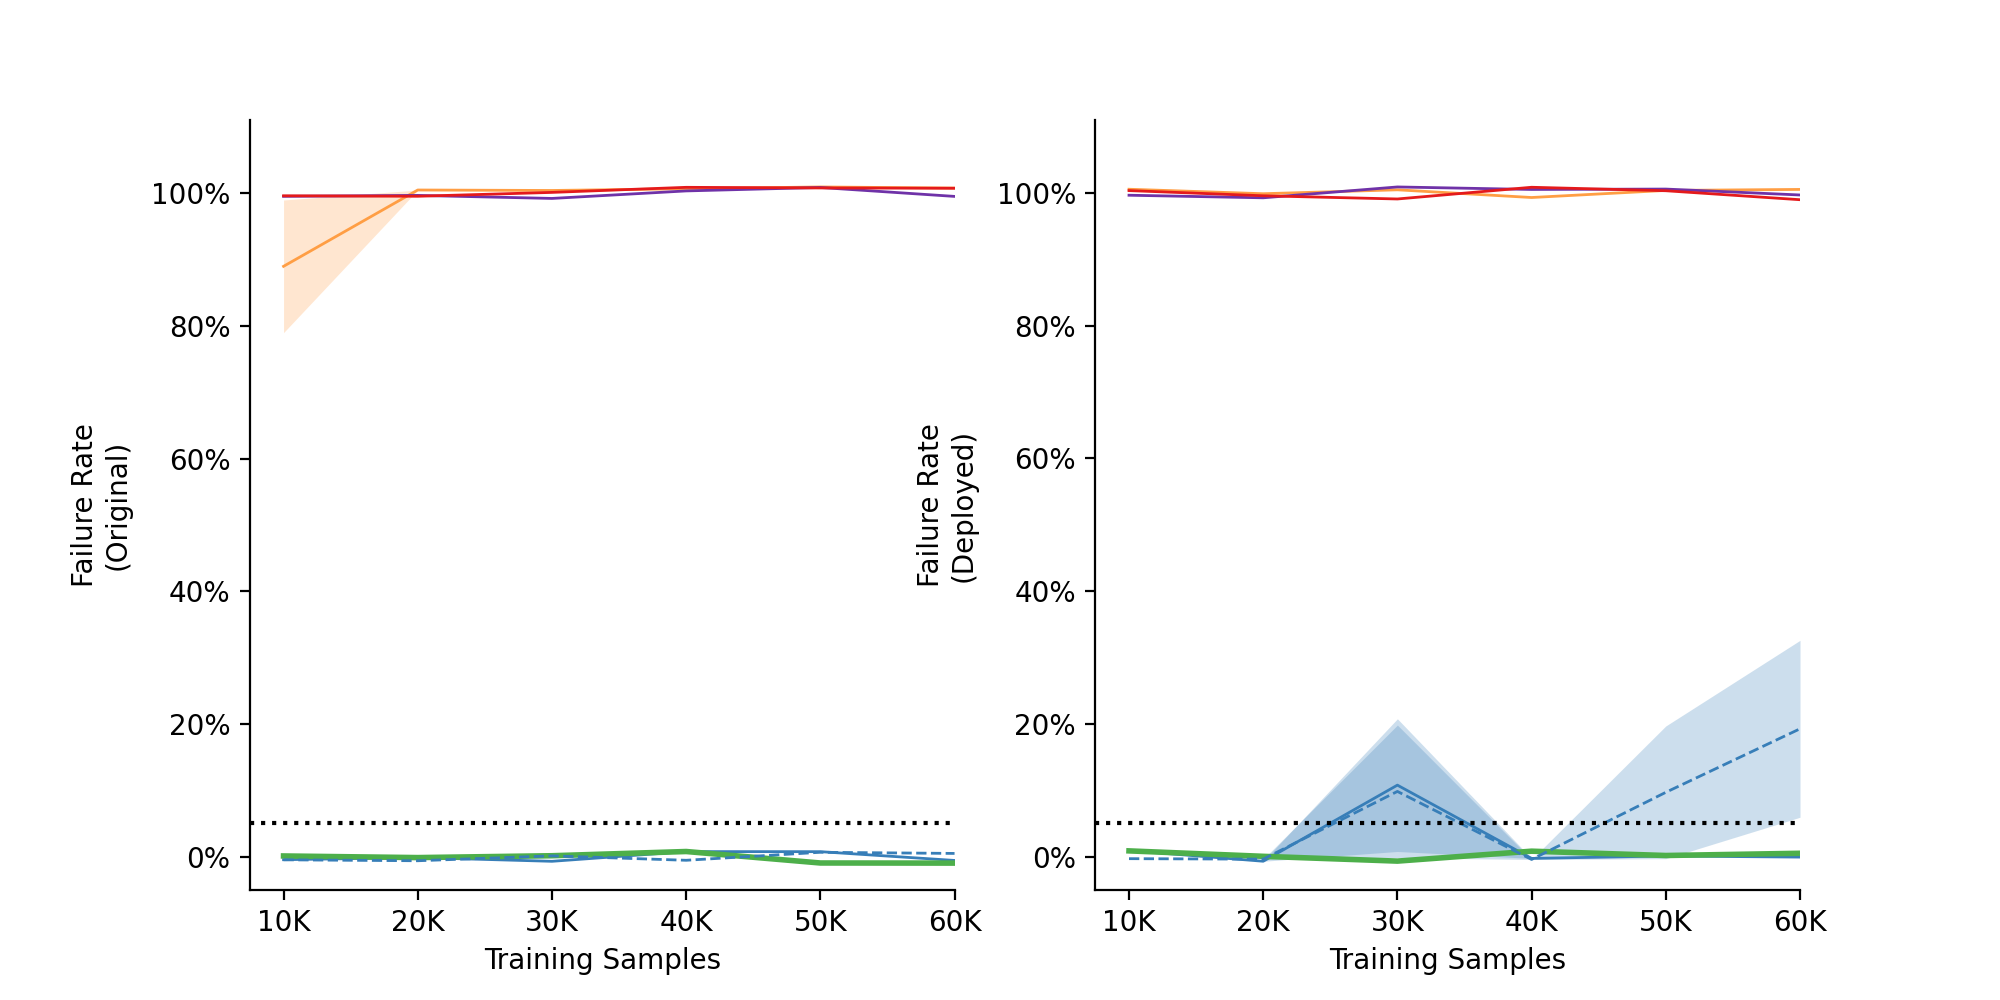
\includegraphics[width=\linewidth]{figures/adult_failure_rates/iclr_adult_antag_ds_rl_di.png}
      \caption{Disparate Impact}
    \end{subfigure}
    \begin{subfigure}{\textwidth}
    \includegraphics[width=\linewidth]{figures/adult_failure_rates/iclr_legend.png}
    \end{subfigure}
    \caption{Failure rates for each algorithm under unknown demographic shift for fairness constraints DP and DI with the \textit{UCI Adult Census} dataset. The confidence bound is indicated with the dotted line.} 
    \label{fig:adult_fr_unk}
\end{figure}


\begin{figure}[ht]
    \begin{subfigure}{0.5\linewidth}
      \centering
      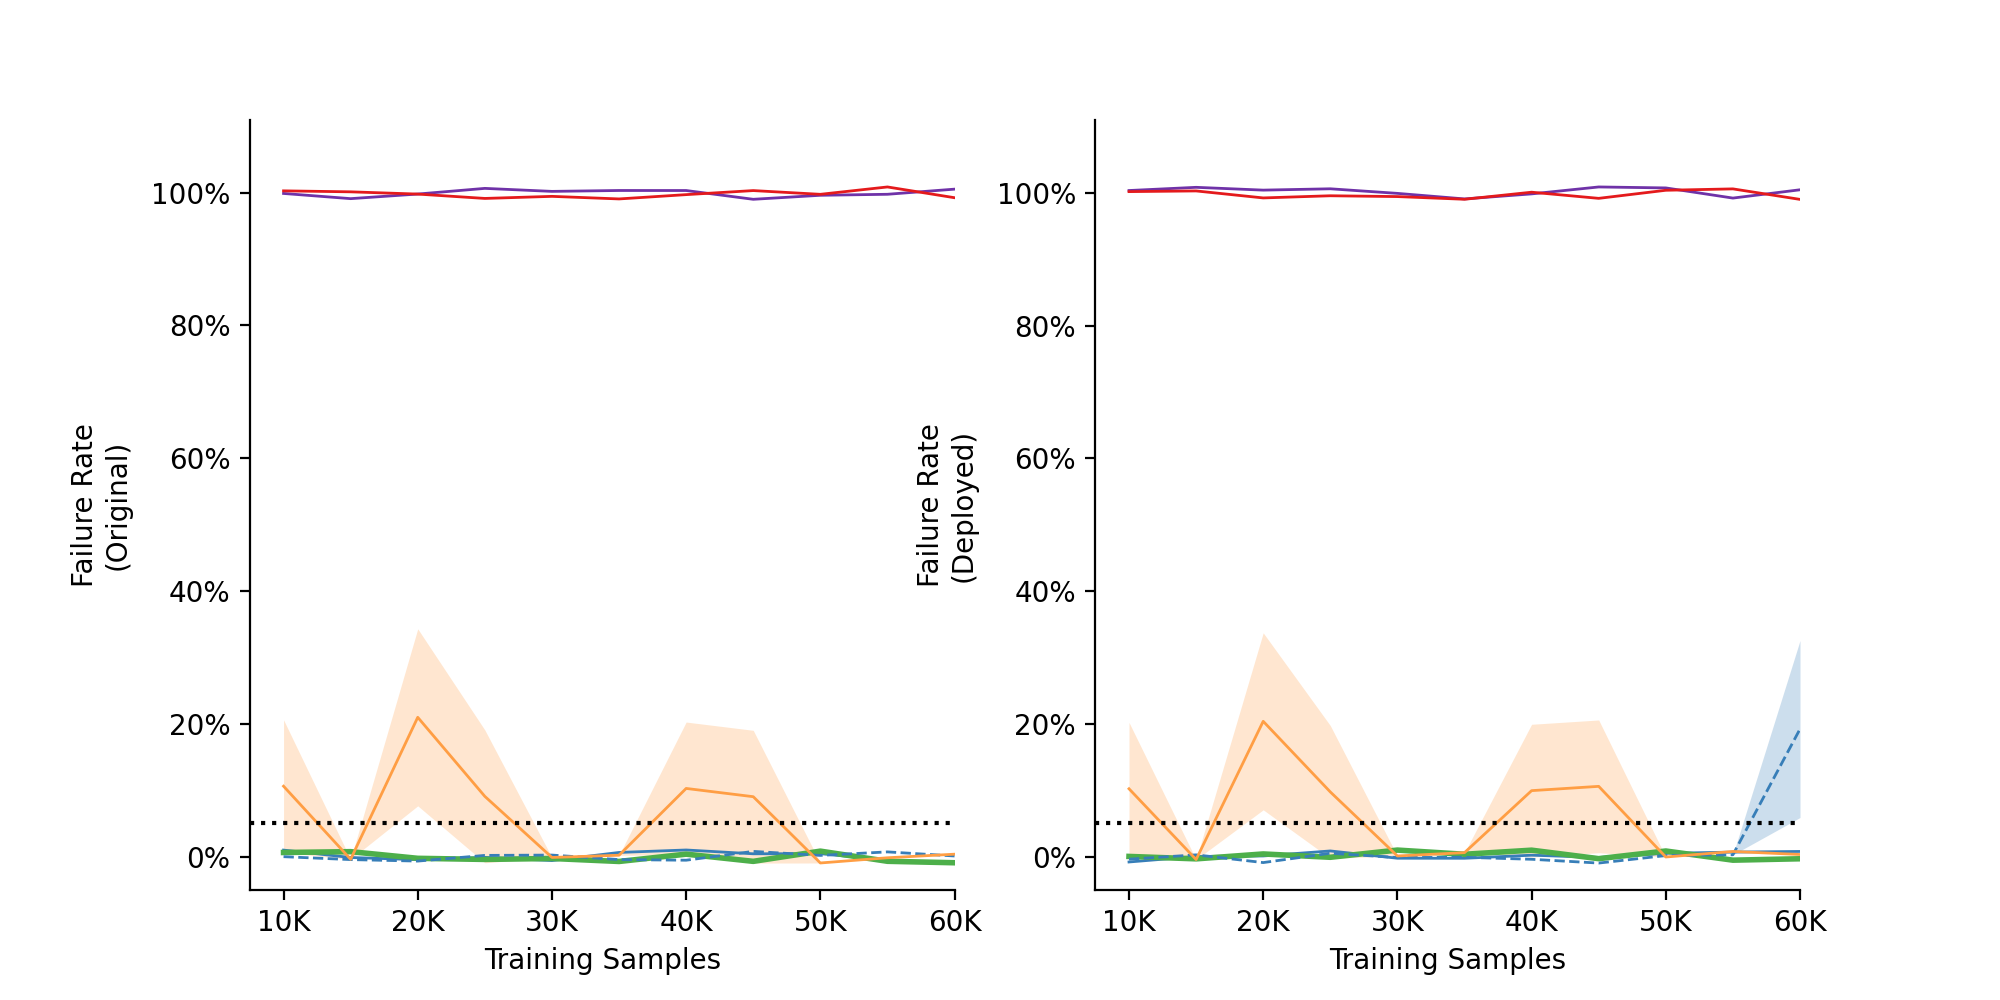
\includegraphics[width=\linewidth]{figures/adult_failure_rates/iclr_adult_fixed_ds_rl_dp.png}
      \caption{Demographic Parity}
    \end{subfigure}
    \begin{subfigure}{0.5\linewidth}
      \centering
      \includegraphics[width=\linewidth]{figures/adult_failure_rates/iclr_adult_fixed_ds_rl_di.png}
      \caption{Disparate Impact}
    \end{subfigure}
    \begin{subfigure}{\textwidth}
    \includegraphics[width=\linewidth]{figures/adult_failure_rates/iclr_legend.png}
    \end{subfigure}
    \caption{Failure rate (in percentages) for each algorithm under known demographic shift for fairness constraints DP and DI with the \textit{UCI Adult Census} dataset. The confidence threshold is indicated with the dotted line.} 
    \label{fig:adult_fr_k}
\end{figure}

\subsection{Numerical Results}\label{sec:app_num_results}
The tables in this section (tables \ref{tab:uci_num_k_DP}, \ref{tab:uci_num_k_DI}, \ref{tab:uci_num_unk_DP}, and \ref{tab:uci_num_unk_DI}) provide numerical results of the accuracy scores on the experiments run with the \textit{UCI Adult Census} dataset, as set out in section \ref{sec:discussion_accuracy}.
\begin{table}[ht] 
\footnotesize 
\begin{tabular}{|c|ccccccccccc|} \hline \multicolumn{12}{|c|}{Accuracy - Known Demographic Shift - Demographic Parity} \\ \hline \hline

Samples & 10k & 15k & 20k & 25k & 30k & 35k & 40k & 45k & 50k & 55k & 60k \\ \hline

\multicolumn{12}{|c|}{Seldonian Classifier} \\ \hline
Original & nan & nan & 76.05 & nan & 76.31 & 76.59 & 76.59 & 77.75 & 78.05 & 78.11 & 78.19 \\ \hline
Deployed & nan & nan & 72.80 & nan & 74.15 & 75.30 & 74.72 & 75.58 & 75.98 & 76.06 & 76.05 \\ \hline 
Difference & nan & nan & -3.25 & nan & -2.16 & -1.29 & -1.87 & -2.17 & -2.07 & -2.05 & -2.14 \\ \hline

\multicolumn{12}{|c|}{Quasi-Seldonian-Robust Classifier (\textbf{\texttt{Shifty}})} \\ \hline
Original & 76.75 & 76.25 & 77.17 & 77.56 & 77.34 & 77.80 & 77.91 & 77.99 & 77.99 & 77.93 & 77.95 \\ \hline
Deployed & 73.60 & 74.11 & 74.37 & 74.99 & 74.66 & 75.19 & 75.62 & 75.44 & 75.53 & 75.72 & 75.73 \\ \hline
Difference & -3.15 & -2.14 & -2.80 & -2.57 & -2.68 & -2.61 & -2.29 & -2.55 & -2.46 & -2.21 & -2.22 \\ \hline

\multicolumn{12}{|c|}{Quasi-Seldonian Classifier} \\ \hline
Original & 76.70 & 77.03 & 77.38 & 78.10 & 78.31 & 78.56 & 78.20 & 78.56 & 78.68 & 78.81 & 78.86 \\ \hline
Deployed & 73.47 & 74.35 & 74.56 & 75.70 & 75.96 & 76.60 & 75.66 & 76.43 & 76.42 & 76.67 & 76.69 \\ \hline
Difference & -3.23 & -2.68 & -2.82 & -2.40 & -2.35 & -1.96 & -2.54 & -2.13 & -2.26 & -2.14 & -2.17 \\ \hline

\multicolumn{12}{|c|}{Fairlearn} \\ \hline
Original & 74.03 & 74.39 & 74.78 & 74.11 & 74.36 & 74.40 & 74.13 & 74.15 & 74.41 & 74.40 & 74.43 \\ \hline
Deployed & 70.91 & 71.24 & 71.76 & 71.04 & 71.23 & 71.25 & 71.05 & 71.06 & 71.25 & 71.25 & 71.26 \\ \hline
Difference & -3.12 & -3.15 & -3.02 & -3.07 & -3.13 & -3.15 & -3.08 & -3.09 & -3.16 & -3.15 & -3.17 \\ \hline 

\multicolumn{12}{|c|}{RFLearn} \\ \hline
Original & 80.99 & 81.03 & 81.01 & 80.92 & 81.05 & 81.00 & 81.03 & 81.04 & 81.12 & 81.02 & 80.98 \\ \hline
Deployed & 78.51 & 78.55 & 78.56 & 78.46 & 78.56 & 78.52 & 78.58 & 78.59 & 78.68 & 78.59 & 78.53 \\ \hline Difference & -2.48 & -2.48 & -2.45 & -2.46 & -2.49 & -2.48 & -2.45 & -2.45 & -2.44 & -2.43 & -2.45 \\ \hline

\multicolumn{12}{|c|}{Fair Constraints} \\ \hline
Original & 80.99 & 80.77 & 80.71 & 80.63 & 80.60 & 80.58 & 80.64 & 80.49 & 80.51 & 80.52 & 80.52 \\ \hline
Deployed & 78.67 & 78.44 & 78.38 & 78.28 & 78.23 & 78.23 & 78.29 & 78.15 & 78.19 & 78.17 & 78.16 \\ \hline
Difference & -2.32 & -2.33 & -2.33 & -2.35 & -2.37 & -2.35 & -2.35 & -2.34 & -2.32 & -2.35 & -2.36 \\ \hline 
\end{tabular}
\caption{Results table showcasing the numerical mean accuracy percentage of each algorithm, for both the original distribution and the deployed one when trained under a known demographic shift with fairness constraint Demographic Parity. The decrease or increase in accuracy is shown in the rows named `Difference'.}
\label{tab:uci_num_k_DP}
\end{table}

\begin{table}[ht]
\footnotesize
\begin{tabular}{|c|ccccccccccc|}
\hline 
\multicolumn{12}{|c|}{Accuracy - Known Demographic Shift - Disparate Impact} \\ \hline \hline

Samples & 10k & 15k & 20k & 25k & 30k & 35k & 40k & 45k & 50k & 55k & 60k \\ \hline

\multicolumn{12}{|c|}{Seldonian Classifier} \\ \hline
Original & 65.00 & 69.93 & 73.23 & 73.60 & 74.40 & 74.96 & 75.30 & 76.72 & 77.01 & 77.01 & 77.65 \\ \hline
Deployed & 65.65 & 69.75 & 71.53 & 72.22 & 73.32 & 73.57 & 73.95 & 75.25 & 75.60 & 75.52 & 76.01 \\ \hline
Difference & 0.65 & -0.18 & -1.70 & -1.38 & -1.08 & -1.39 & -1.35 & -1.47 & -1.41 & -1.49 & -1.64 \\ \hline
  
\multicolumn{12}{|c|}{Quasi-Seldonian-Robust Classifier (\textbf{\texttt{Shifty}})} \\ \hline
Original & 67.31 & 68.49 & 71.50 & 74.14 & 74.58 & 76.98 & 77.01 & 76.90 & 77.03 & 77.32 & 77.29 \\ \hline
Deployed & 67.30 & 66.93 & 69.81 & 72.72 & 72.79 & 75.45 & 75.49 & 74.69 & 74.70 & 75.16 & 75.33 \\ \hline
Difference & -0.01 & -1.56 & -1.69 & -1.42 & -1.79 & -1.53 & -1.52 & -2.21 & -2.33 & -2.16 & -1.96 \\ \hline

\multicolumn{12}{|c|}{Quasi-Seldonian Classifier} \\ \hline
Original & 66.72 & 71.57 & 72.95 & 76.02 & 75.96 & 76.90 & 77.65 & 77.69 & 78.20 & 78.42 & 78.49 \\ \hline
Deployed & 66.92 & 69.32 & 72.21 & 74.55 & 74.05 & 74.91 & 75.77 & 75.80 & 76.38 & 76.87 & 76.70 \\ \hline
Difference & 0.20 & -2.25 & -0.74 & -1.47 & -1.91 & -1.99 & -1.88 & -1.89 & -1.82 & -1.55 & -1.79 \\ \hline

\multicolumn{12}{|c|}{Fairlearn} \\ \hline
Original & 80.10 & 79.77 & 79.94 & 80.60 & 80.58 & 80.68 & 80.61 & 80.68 & 80.68 & 80.68 & 80.66 \\ \hline
Deployed & 77.54 & 77.20 & 77.35 & 78.09 & 78.12 & 78.16 & 78.11 & 78.15 & 78.15 & 78.13 & 78.12 \\ \hline
Difference & -2.56 & -2.57 & -2.59 & -2.51 & -2.46 & -2.52 & -2.50 & -2.53 & -2.53 & -2.55 & -2.54 \\ \hline

\multicolumn{12}{|c|}{RFLearn} \\ \hline
Original & 81.00 & 81.05 & 81.07 & 81.08 & 81.01 & 81.00 & 80.98 & 81.07 & 80.97 & 81.03 & 80.99 \\ \hline
Deployed & 78.58 & 78.64 & 78.64 & 78.67 & 78.58 & 78.54 & 78.54 & 78.64 & 78.53 & 78.61 & 78.54 \\ \hline
Difference & -2.42 & -2.41 & -2.43 & -2.41 & -2.43 & -2.46 & -2.44 & -2.43 & -2.44 & -2.42 & -2.45 \\ \hline

\multicolumn{12}{|c|}{Fair Constraints} \\ \hline
Original & 81.04 & 81.14 & 80.66 & 80.61 & 80.64 & 80.64 & 80.69 & 80.61 & 80.63 & 80.54 & 80.58 \\ \hline
Deployed & 78.70 & 78.81 & 78.33 & 78.27 & 78.28 & 78.27 & 78.34 & 78.25 & 78.27 & 78.16 & 78.21 \\ \hline
Difference & -2.34 & -2.33 & -2.33 & -2.34 & -2.36 & -2.37 & -2.35 & -2.36 & -2.36 & -2.38 & -2.37 \\ \hline

\end{tabular}
\caption{Results table showcasing the numerical mean accuracy percentage of each algorithm, for both the original distribution and the deployed one when trained under a known demographic shift with fairness constraint Disparate Impact. The decrease or increase in accuracy are shown per number of samples in the rows named `Difference'}
\label{tab:uci_num_k_DI}
\end{table}

\begin{table}[ht]
\footnotesize
\centering
\begin{tabular}{|c|cccccc|}
\hline
\multicolumn{7}{|c|}{Accuracy - Unknown Demographic Shift - Demographic Parity} \\ \hline

Samples & 10k & 20k & 30k & 40k & 50k & 60k \\ \hline

\multicolumn{7}{|c|}{Seldonian Classifier} \\ \hline
Original & 77.23 & 78.74 & 79.40 & 79.54 & 79.75 & 80.08 \\ \hline
Deployed & 76.31 & 77.06 & 77.49 & 77.67 & 77.93 & 78.03 \\ \hline
Difference & -0.92 & -1.68 & -1.91 & -1.87 & -1.82 & -2.05 \\ \hline

\multicolumn{7}{|c|}{Quasi-Seldonian-Robust Classifier (\textbf{\texttt{Shifty}})} \\ \hline
Original & 78.39 & 79.23 & 79.32 & 79.65 & 79.66 & 79.83 \\ \hline 
Deployed & 76.95 & 77.29 & 77.39 & 77.61 & 77.71 & 77.88 \\ \hline 
Difference & -1.44 & -1.94 & -1.93 & -2.04 & -1.95 & -1.95 \\ \hline

\multicolumn{7}{|c|}{Quasi-Seldonian Classifier} \\ \hline
Original & 78.85 & 79.70 & 80.28 & 80.49 & 80.61 & 80.68 \\ \hline
Deployed & 76.65 & 77.68 & 78.16 & 78.29 & 78.36 & 78.46 \\ \hline
Difference & -2.20 & -2.02 & -2.12 & -2.20 & -2.25 & -2.22 \\ \hline

\multicolumn{7}{|c|}{Fairlearn} \\ \hline
Original & 75.03 & 75.03 & 74.38 & 74.40 & 75.07 & 75.05 \\ \hline
Deployed & 72.17 & 72.17 & 71.47 & 71.47 & 72.19 & 72.19 \\ \hline
Difference & -2.86 & -2.86 & -2.91 & -2.93 & -2.88 & -2.86 \\ \hline

\multicolumn{7}{|c|}{RFLearn} \\ \hline
Original & 80.97 & 80.92 & 80.94 & 80.86 & 80.86 & 80.89 \\ \hline 
Deployed & 78.73 & 78.66 & 78.70 & 78.61 & 78.61 & 78.62 \\ \hline
Difference & -2.24 & -2.26 & -2.24 & -2.25 & -2.25 & -2.27 \\ \hline

\multicolumn{7}{|c|}{Fair Constraints} \\ \hline 
Original & 81.02 & 80.67 & 80.69 & 80.63 & 80.60 & 80.58 \\ \hline
Deployed & 78.84 & 78.47 & 78.51 & 78.46 & 78.42 & 78.41 \\ \hline
Difference & -2.18 & -2.20 & -2.18 & -2.17 & -2.18 & -2.17 \\ \hline
\end{tabular}
\caption{Results table showcasing the numerical mean accuracy percentage of each algorithm, for both the original distribution and the deployed one when trained under an unknown demographic shift with fairness constraint Demographic Parity. The decrease or increase in accuracy is shown in the rows named `Difference'.}
\label{tab:uci_num_unk_DP}
\end{table}

\begin{table}[ht]
\footnotesize
\centering
\begin{tabular}{|c|cccccc|}
\hline
\multicolumn{7}{|c|}{Accuracy - Unknown Demographic Shift - Disparate Impact} \\ \hline \hline

Samples & 10k & 20k & 30k & 40k & 50k & 60k \\ \hline

\multicolumn{7}{|c|}{Seldonian Classifier} \\ 
\hline Original & 64.66 & 71.92 & 75.22 & 75.74 & 77.17 & 76.74 \\ \hline
Deployed & 65.43 & 71.93 & 75.63 & 76.54 & 80.18 & 79.55 \\ \hline
Difference & 0.77 & 0.01 & 0.41 & 0.80 & 3.01 & 2.81 \\ \hline

\multicolumn{7}{|c|}{Quasi-Seldonian-Robust Classifier (\textbf{\texttt{Shifty}})} \\ \hline 
Original & 52.97 & nan & 73.30 & 75.09 & 75.61 & 76.39 \\ \hline
Deployed & 52.36 & nan & 73.20 & 74.29 & 74.40 & 74.71 \\ \hline
Difference & -0.61 & nan & -0.10 & -0.80 & -1.21 & -1.68 \\ \hline 

\multicolumn{7}{|c|}{Quasi-Seldonian Classifier} \\ \hline
Original & 67.03 & 74.15 & 76.09 & 77.71 & 77.41 & 78.17 \\ \hline
Deployed & 67.31 & 75.56 & 76.82 & 79.09 & 79.14 & 78.73 \\ \hline
Difference & 0.28 & 1.41 & 0.73 & 1.38 & 1.73 & 0.56 \\ \hline

\multicolumn{7}{|c|}{Fairlearn} \\ \hline
Original & 80.01 & 80.00 & 80.68 & 80.68 & 80.68 & 80.69 \\ \hline
Deployed & 82.78 & 82.78 & 84.24 & 84.34 & 84.15 & 84.54 \\ \hline
Difference & 2.77 & 2.78 & 3.56 & 3.66 & 3.47 & 3.85 \\ \hline

\multicolumn{7}{|c|}{RFLearn} \\ \hline
Original & 81.00 & 80.95 & 80.98 & 80.96 & 81.03 & 80.98 \\ \hline
Deployed & 83.06 & 83.26 & 82.14 & 82.60 & 82.00 & 82.69 \\ \hline
Difference & 2.06 & 2.31 & 1.16 & 1.64 & 0.97 & 1.71 \\ \hline

\multicolumn{7}{|c|}{Fair Constraints} \\ \hline
Original & 80.97 & 80.65 & 80.64 & 80.55 & 80.65 & 80.52 \\ \hline
Deployed & 81.78 & 80.00 & 79.97 & 79.15 & 79.56 & 79.37 \\ \hline 
Difference & 0.81 & -0.65 & -0.67 & -1.40 & -1.09 & -1.15 \\ \hline

\end{tabular}
\caption{Results table showcasing the numerical mean accuracy percentage of each algorithm, for both the original distribution and the deployed one when trained under an unknown demographic shift with fairness constraint Disparate Impact. The decrease or increase in accuracy is shown in the rows named `Difference'.}
\label{tab:uci_num_unk_DI}
\end{table}